\documentclass[tikz, border=10pt]{standalone}
\usepackage{tikz}
\usetikzlibrary{calc}

\begin{document}

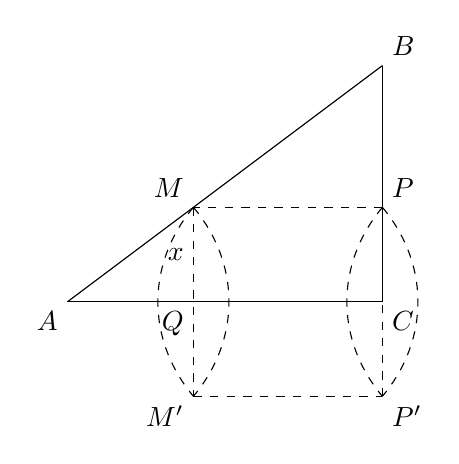
\begin{tikzpicture}
    \coordinate (A) at (0,0);
    \coordinate (B) at (4,3);
    \coordinate (C) at (4,0);

    \coordinate (M) at (1.6,1.2);
    \coordinate (P) at (4,1.2);
    \coordinate (Q) at (1.6,0);

    \coordinate (M') at (1.6,-1.2);
    \coordinate (P') at (4,-1.2);

    \draw[black] (A) to (B);
    \draw[black] (B) to (C);
    \draw[black] (A) to (C);
    \draw[dashed, black] (P) to (M);
    \draw[dashed, black] (M) to (M');
    \draw[dashed, black] (M') to (P');
    \draw[dashed, black] (P') to (C);
    \draw[dashed, black] (M) to [out=-130, in=130] (M');
    \draw[dashed, black] (M) to [out=-50, in=50] (M');
    \draw[dashed, black] (P) to [out=-130, in=130] (P');
    \draw[dashed, black] (P) to [out=-50, in=50] (P');
    
    \node[below left]  at (A) {$A$};
    \node[above right] at (B) {$B$};
    \node[below right] at (C) {$C$};

    \node[above left] at (M) {$M$};
    \node[above right] at (P) {$P$};
    \node[below left] at (Q) {$Q$};
    
    \node[below left] at (M') {$M'$};
    \node[below right] at (P') {$P'$};

    \node[left] at ($(M)!0.5!(Q)$) {$x$};
\end{tikzpicture}

\end{document}
